\begin{figure*}[t]
    \centering
    \definecolor{figBlue}{HTML}{2166AC}\definecolor{figRed}{HTML}{B2182B}\definecolor{figInk}{HTML}{1D2329}\definecolor{figMuted}{HTML}{6B7580}
    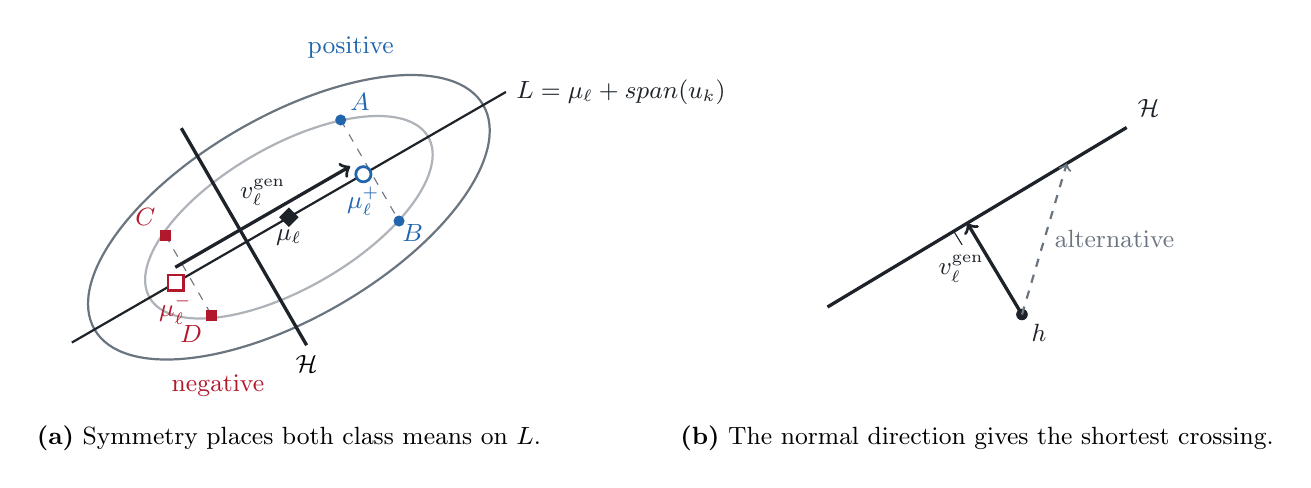
\begin{tikzpicture}[scale=0.95, every node/.style={font=\small},
        posPt/.style={circle, fill=figBlue, inner sep=0pt, minimum size=4pt},
        negPt/.style={rectangle, fill=figRed, inner sep=0pt, minimum size=4pt},
        posMean/.style={circle, draw=figBlue, fill=white, line width=1pt, inner sep=0pt, minimum size=5.5pt},
        negMean/.style={rectangle, draw=figRed, fill=white, line width=1pt, inner sep=0pt, minimum size=5.5pt},
        centrePt/.style={rectangle, rotate=45, fill=figInk, inner sep=0pt, minimum size=5pt}]
        \begin{scope}[xshift=-4.6cm]
          \begin{scope}[rotate=30]
            \draw[figMuted, thick] (0,0) ellipse (3.0 and 1.35);
            \draw[figMuted!55, thick] (0,0) ellipse (2.15 and 0.95);
            \draw[figInk, thick] (-3.35,0) -- (3.35,0)
                node[right] {$L=\mu_\ell+\operatorname{span}(u_k)$};
            \draw[figInk, very thick] (-0.65,-1.60) -- (-0.65,1.75);
            \node[below] at (-0.65,-1.60)
                {$\mathcal{H}$};
            \node[figBlue] at (1.85,1.55) {positive};
            \node[figRed] at (-1.95,-1.48) {negative};

            \draw[figMuted, dashed] (1.25,0.78) -- (1.25,-0.78);
            \draw[figMuted, dashed] (-1.55,0.62) -- (-1.55,-0.62);
            \node[posPt] at (1.25,0.78) {};
            \node[above right, figBlue] at (1.25,0.78) {$A$};
            \node[posPt] at (1.25,-0.78) {};
            \node[below right, inner sep=1pt, figBlue] at (1.25,-0.78) {$B$};
            \node[negPt] at (-1.55,0.62) {};
            \node[above left, figRed] at (-1.55,0.62) {$C$};
            \node[negPt] at (-1.55,-0.62) {};
            \node[below left, figRed] at (-1.55,-0.62) {$D$};

            \node[centrePt] at (0,0) {};
            \node[below=1pt, figInk] at (0,0) {$\mu_\ell$};
            \node[negMean] at (-1.75,0) {};
            \node[below=1pt, figRed] at (-1.75,0) {$\mu_\ell^{-}$};
            \node[posMean] at (1.15,0) {};
            \node[below=1pt, figBlue] at (1.15,0) {$\mu_\ell^{+}$};
            \draw[figInk, ->, very thick] (-1.65,0.18) -- (1.05,0.18)
                node[midway, above] {$v_\ell^{\mathrm{gen}}$};
          \end{scope}
            \node at (0,-2.95) {\textbf{(a)} Symmetry places both class means on $L$.};
        \end{scope}

        \begin{scope}[xshift=4.6cm]
            \draw[figInk, very thick] (-2.0,-1.20) -- (2.0,1.20)
                node[above right] {$\mathcal{H}$};
            \fill[figInk] (0.60,-1.30) circle (2.2pt) node[below right] {$h$};
            \draw[figInk, ->, very thick] (0.60,-1.30) -- (-0.13,-0.08)
                node[midway, left] {$v_\ell^{\mathrm{gen}}$};
            \draw[figMuted, ->, dashed, thick] (0.60,-1.30) -- (1.20,0.72)
                node[midway, right] {alternative};
            \draw[figInk] (-0.13,-0.08) -- (-0.31,-0.19) -- (-0.20,-0.37);
            \node at (0,-2.95) {\textbf{(b)} The normal direction gives the shortest crossing.};
        \end{scope}
    \end{tikzpicture}
    \caption{Geometric proof idea for genesis steering under principal-axis
    separability. Circles denote the positive class and squares the negative
    class; filled markers are sample points and hollow markers are the class
    means. The dark point $\mu_\ell$ is the center of the overall
    representation distribution, $L$ is the separating principal axis, and
    $\mathcal{H}$ is the linear separator. In an elliptically symmetric
    density, equal-density points can be paired across $L$, so their components
    perpendicular to $L$ cancel in expectation. The resulting mean-difference
    direction is normal to $\mathcal{H}$, which is also the shortest direction
    for crossing it.}
    \label{fig:genesis-geometry}
\end{figure*}

\begin{comment}

\begin{figure*}[t]
    \centering
    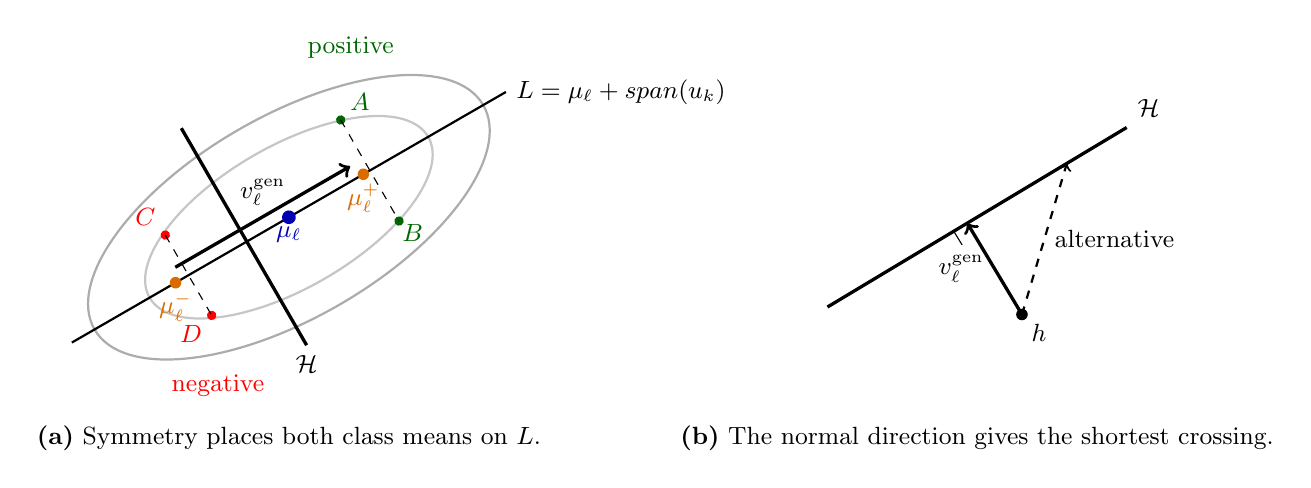
\begin{tikzpicture}[scale=0.95, every node/.style={font=\small}]
        \begin{scope}[xshift=-4.6cm]
          \begin{scope}[rotate=30]
            \draw[gray!65, thick] (0,0) ellipse (3.0 and 1.35);
            \draw[gray!45, thick] (0,0) ellipse (2.15 and 0.95);
            \draw[black, thick] (-3.35,0) -- (3.35,0)
                node[right] {$L=\mu_\ell+\operatorname{span}(u_k)$};
            \draw[black, very thick] (-0.65,-1.60) -- (-0.65,1.75);
            \node[below] at (-0.65,-1.60)
                {$\mathcal{H}$};
            \node[green!40!black] at (1.85,1.55) {positive};
            \node[red] at (-1.95,-1.48) {negative};

            \fill[green!40!black] (1.25,0.78) circle (1.8pt) node[above right, green!40!black] {$A$};
            \fill[green!40!black] (1.25,-0.78) circle (1.8pt) node[below right, inner sep=1pt, green!40!black] {$B$};
            \draw[dashed] (1.25,0.78) -- (1.25,-0.78);
            \fill[red] (-1.55,0.62) circle (1.8pt) node[above left, red] {$C$};
            \fill[red] (-1.55,-0.62) circle (1.8pt) node[below left, red] {$D$};
            \draw[dashed] (-1.55,0.62) -- (-1.55,-0.62);

            \fill[blue!70!black] (0,0) circle (2.6pt)
                node[below, blue!70!black] {$\mu_\ell$};
            \fill[orange!85!black] (-1.75,0) circle (2.2pt)
                node[below, orange!85!black] {$\mu_\ell^{-}$};
            \fill[orange!85!black] (1.15,0) circle (2.2pt)
                node[below, orange!85!black] {$\mu_\ell^{+}$};
            \draw[->, very thick] (-1.65,0.18) -- (1.05,0.18)
                node[midway, above] {$v_\ell^{\mathrm{gen}}$};
          \end{scope}
            \node at (0,-2.95) {\textbf{(a)} Symmetry places both class means on $L$.};
        \end{scope}

        \begin{scope}[xshift=4.6cm]
            \draw[black, very thick] (-2.0,-1.20) -- (2.0,1.20)
                node[above right] {$\mathcal{H}$};
            \fill (0.60,-1.30) circle (2.2pt) node[below right] {$h$};
            \draw[->, very thick] (0.60,-1.30) -- (-0.13,-0.08)
                node[midway, left] {$v_\ell^{\mathrm{gen}}$};
            \draw[->, dashed, thick] (0.60,-1.30) -- (1.20,0.72)
                node[midway, right] {alternative};
            \draw (-0.13,-0.08) -- (-0.31,-0.19) -- (-0.20,-0.37);
            \node at (0,-2.95) {\textbf{(b)} The normal direction gives the shortest crossing.};
        \end{scope}
    \end{tikzpicture}
    \caption{Geometric proof idea for genesis steering under principal-axis
    separability. The blue point $\mu_\ell$ is the center of the overall
    representation distribution, $L$ is the separating principal axis, and
    $\mathcal{H}$ is the linear separator. In an elliptically symmetric
    density, equal-density points can be paired across $L$, so their components
    perpendicular to $L$ cancel in expectation. The resulting mean-difference
    direction is normal to $\mathcal{H}$, which is also the shortest direction
    for crossing it.}
    \label{fig:genesis-geometry}
\end{figure*}

\end{comment}